%\documentclass[11pt, twoside, b5paper]{book}
\documentclass[11pt, twoside, b5paper]{extbook}

\usepackage[b5paper, margin=2cm, innermargin=2cm]{geometry}
%\usepackage[b5paper]{geometry}
%\geometry{verbose, tmargin=1.9cm, bmargin=1.9cm, lmargin=1.9cm, rmargin=1.2cm}

%\usepackage{bera}
\usepackage{fancyhdr}
\usepackage[Bjornstrup]{fncychap}

\pagestyle{plain}

\usepackage{emptypage}
\usepackage{subfiles}
\usepackage{color}
\definecolor{mygray}{gray}{0.75}
\definecolor{dkblue}{rgb}{0,0,0.4}
\usepackage{xcolor}

\usepackage{imakeidx}
\usepackage{hyperref}
\makeindex[name=authors,title=Authors,intoc=true]
\hypersetup{pdftitle={IPMU 2020 Book of abstracts},
 pdfauthor={Fernando Batista},
 pdfsubject={IPMU 2020},
 pdfkeywords={IPMU 2020, book of abstracts},
 colorlinks, citecolor=dkblue, filecolor=dkblue, linkcolor=dkblue, urlcolor=blue}

\usepackage[utf8]{inputenc}
\usepackage[T1]{fontenc}

\usepackage{eurosym}
\usepackage{amsfonts, amsmath, hanging, parskip, times}
\usepackage[numbers]{natbib}
\usepackage[pdftex]{graphicx}

\usepackage{pdfpages}

\newcommand\keywords[1]{%
    \begingroup
    \def\and{-- }
    \par
    \noindent\textbf{Keywords: } #1\par
    \endgroup
}

\providecommand{\tightlist}{%
	\setlength{\itemsep}{0pt}\setlength{\parskip}{0pt}}

\setcounter{secnumdepth}{0}
\setcounter{tocdepth}{3}

\usepackage{titlesec}

%\titleformat{\chapter}[display]{\normalfont\huge\bfseries}{\chaptertitlename\ \thechapter}{20pt}{\Huge}   
%\titlespacing*{\chapter}{0pt}{-50pt}{40pt}
% \titleformat{\chapter}[display]{\normalfont\bfseries}{}{0pt}{\Large}

%\titleformat{\section}[block]{\Large\bfseries}{}{0pt}{\\}[\vspace{2pt}]
\titleformat{\section}[block]{\Large\bfseries\filcenter}{}{1em}{}

\newcommand{\colorsection}[1]{%
  \colorbox{blue!15}{\parbox[b][2.5cm]{\dimexpr\textwidth-2\fboxsep}{\begin{flushright}#1\end{flushright}\vspace{6pt}}}}

\titleformat{name=\chapter}[block]{\sffamily\bfseries\Large}{}{0pt}{\colorsection}  
\titlespacing*{\chapter}{0pt}{\baselineskip}{40pt}

\newcommand{\mychapter}[1]{
	\chapter*{#1}
    	\phantomsection
	\addcontentsline{toc}{chapter}{#1}
	\markboth{#1}{#1}%
}

\usepackage{array}
\providecommand{\tabularnewline}{\\}

\title{IPMU 2020 \\
18th International Conference on Information Processing and Management of Uncertainty in Knowledge-Based Systems}
\author{June 15th – 19th 2020, Lisbon, Portugal}
\date{}

\begin{document}

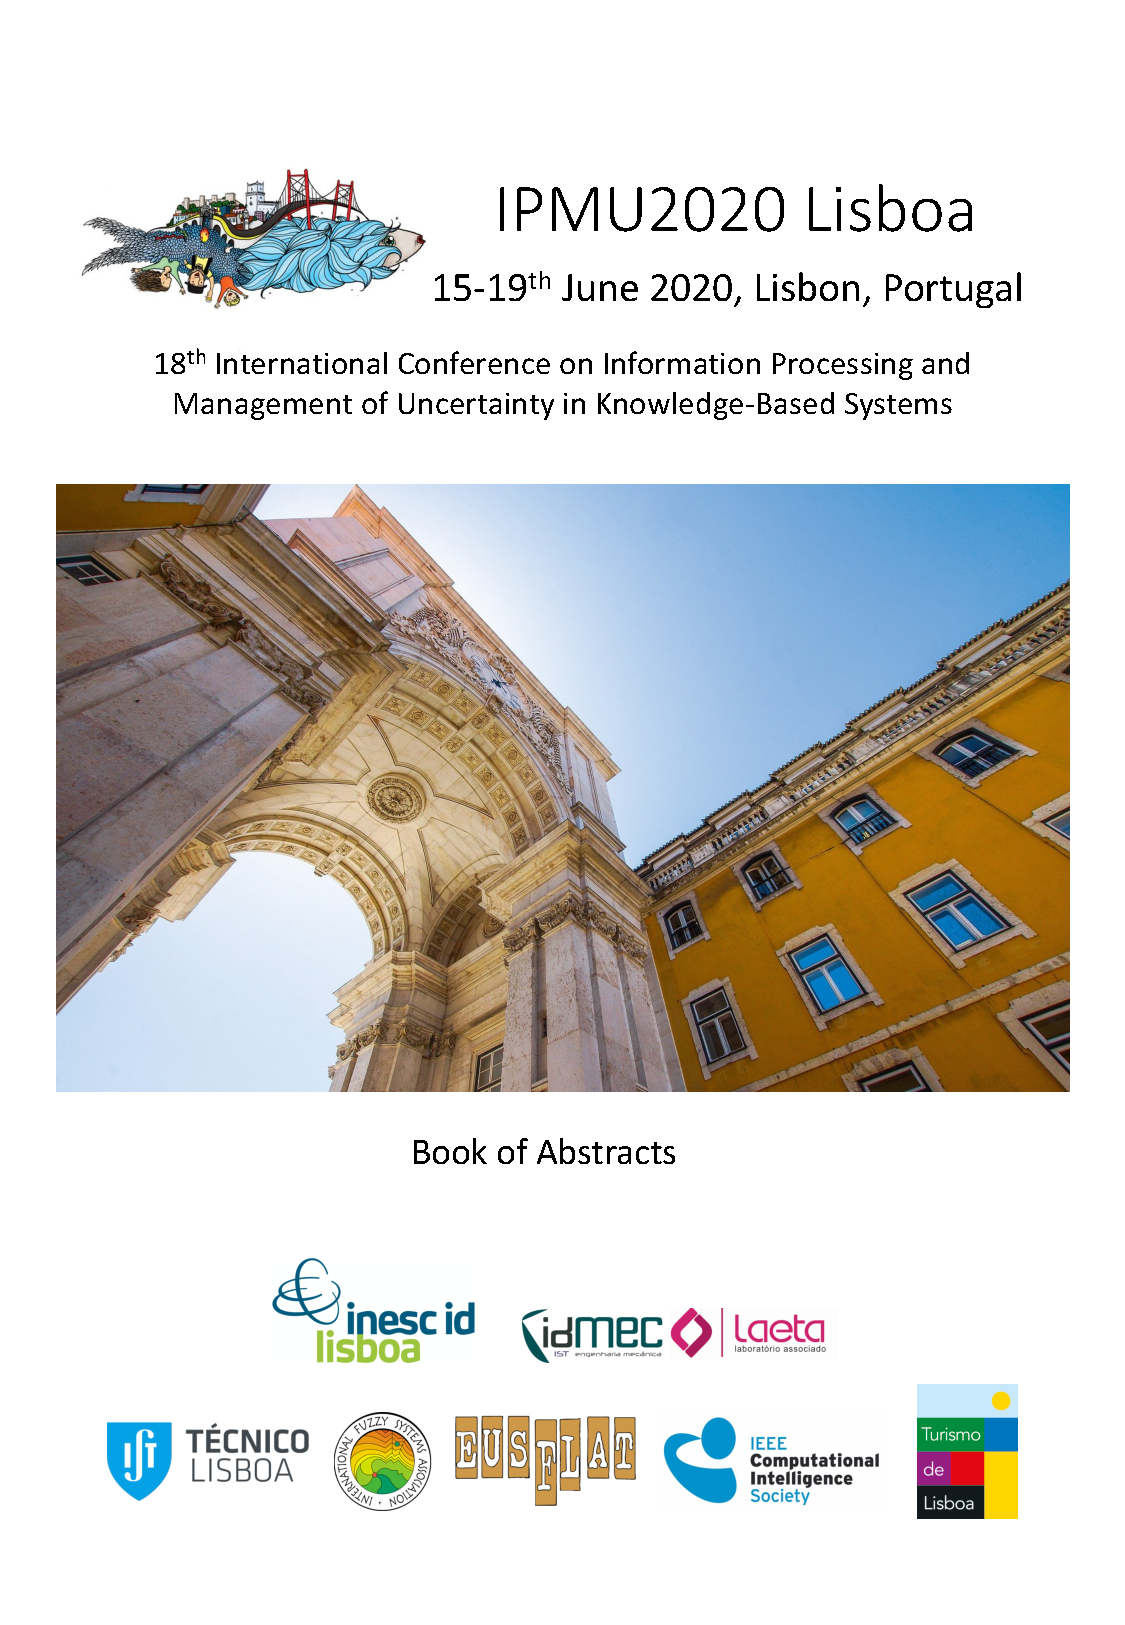
\includepdf{images/front_cover.pdf}
% \cleardoublepage

\clearpage

\frontmatter
\maketitle

\begin{small}
\tableofcontents
\end{small}

\mainmatter

\mychapter{The Organizing Committee}

\subsection*{General Chair}

Joao Paulo Carvalho (Portugal)

\subsection*{Program Chairs}

Marek Reformat (Canada)\\
Marie-Jeanne Lesot (France)\\
Susana Vieira (Portugal)

\subsection*{Publication Chair}

Anna Wilbik (Netherlands)

\subsection*{Special Session Chair}

Uzay Kaymak (Netherlands)

\subsection*{Sponsors and Publicity Chair}

João M. C. Sousa (Portugal)

\subsection*{Web Chair}

Fernando Batista (Portugal)

\subsection*{Executive directors}

Bernadette BOUCHON-MEUNIER\\
Ronald R. YAGER

%\chapter{Welcome to IPMU 2020}
%\input{misc/welcome.tex}

%\chapter{List of venues}
%\input{misc/venues.tex}

%\chapter*{Program overview}
%\addcontentsline{toc}{chapter}{Program overview}

\mychapter{Program overview}

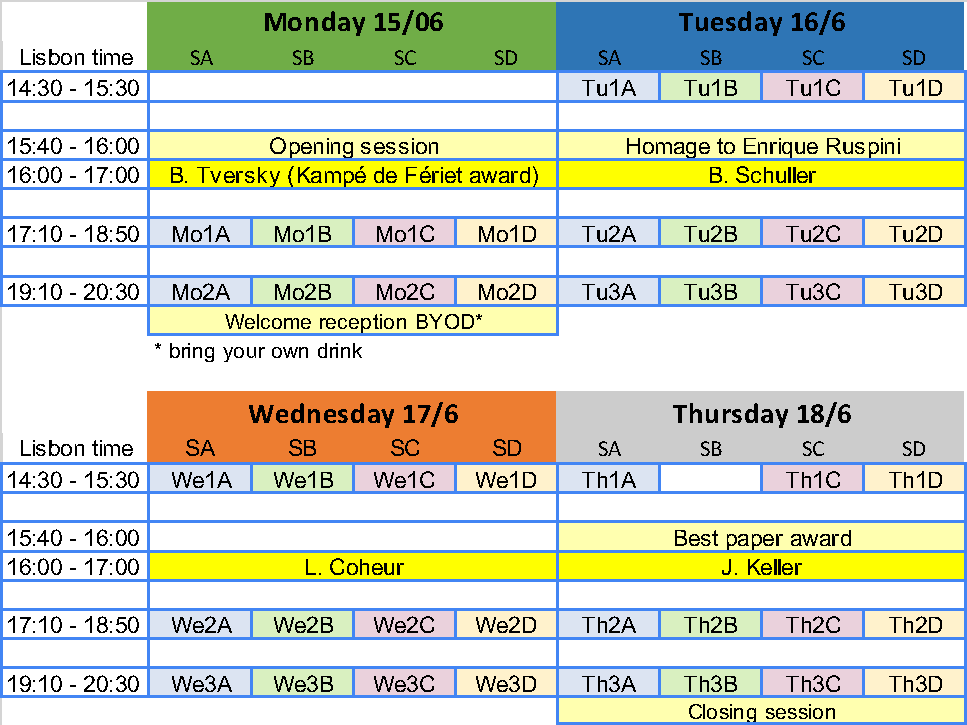
\includegraphics[width=1\textwidth]{images/program_overview.pdf}

%\noindent\makebox[\textwidth]{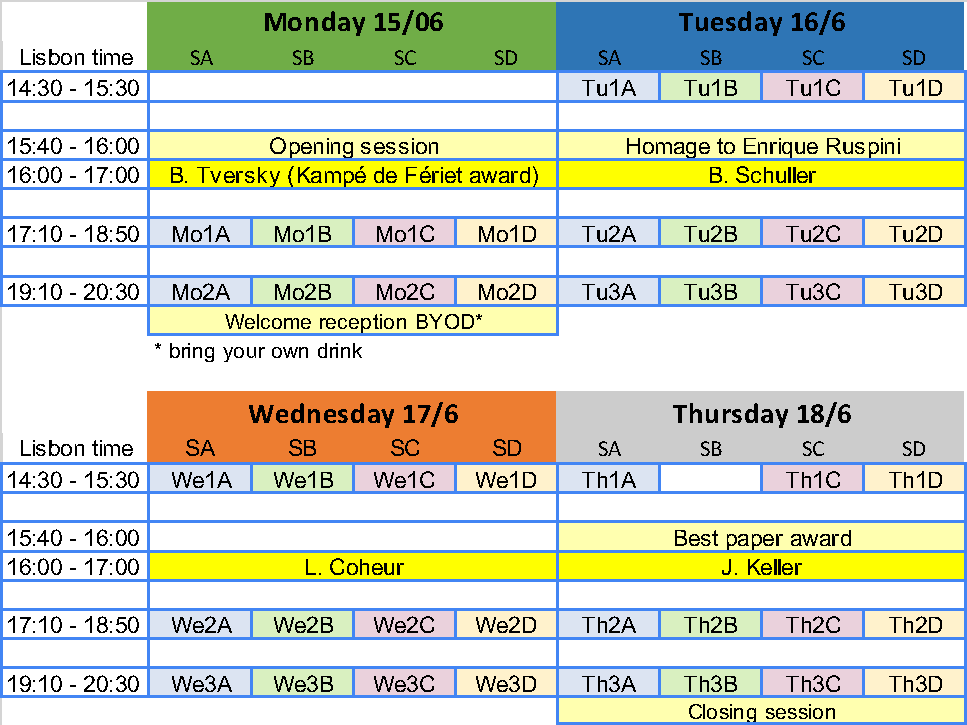
\includegraphics[width=1.25\textwidth,trim=0cm 14cm 0cm 0cm,clip]{images/program_overview.pdf}}
%\begin{flushright}
%\includegraphics[width=0.25\textwidth,trim=0cm 1cm 1cm 0cm,clip]{figs/qrcode}
%\end{flushright}

\mychapter{Full Program}
%\input{misc/program-overview.tex}

\section{Thursday, 16}

\begin{center}
\resizebox{\textwidth}{!}{%%
\small
\begin{tabular}{|c|>{\centering}p{0.2\columnwidth}|>{\centering}p{0.2\columnwidth}|>{\centering}p{0.2\columnwidth}|>{\centering}p{0.2\columnwidth}|}
\hline 
14:30 - 15:30 & Image Processing & SS21: Formal Concept Analysis, Rough Sets, General Operators and Related
Topics, part I & SS9: Computational Intelligence for Logistics and Transportation Problems & SS11: Soft Methods in Statistics and Data Analysis, part II\tabularnewline
\hline 
15:40 - 16:00 & \multicolumn{4}{c|}{Homage to Enrique Ruspini}\tabularnewline
\hline 
16:00 - 17:00 & \multicolumn{4}{c|}{B. Schuller}\tabularnewline
\hline 
17:10 - 18:50 & Decision making, preference \& votes & SS5: Aggregation: Theory and Practice, part I & SS15: Mathematical Methods Towards Dealing with Uncertainty in Applied
Sciences, part I & SS16: Statistical Image Processing and Analysis, with Applications
in Neuroimaging\tabularnewline
\hline 
19:10 - 20:30 & SS2: Theoretical and Applied Aspects of Imprecise Probabilities, part
III & SS5: Aggregation: Theory and Practice, part II & Temporal Data Processing & SS20: Mathematical Fuzzy Logic and Graded Reasoning Models, part I\tabularnewline
\hline 
\end{tabular}}
\par\end{center}

\section{Thursday, 15}
Invited Talks
Session PresenterName  PaperTitle Chairman\\
Session PresenterName  PaperTitle Chairman\\
Session PresenterName  PaperTitle Chairman\\
Session PresenterName  PaperTitle Chairman\\
Session PresenterName  PaperTitle Chairman\\
Session PresenterName  PaperTitle Chairman\\
Session PresenterName  PaperTitle Chairman\\
Session PresenterName  PaperTitle Chairman\\
Session PresenterName  PaperTitle Chairman\\
Session PresenterName  PaperTitle Chairman\\
Session PresenterName  PaperTitle Chairman\\
Session PresenterName  PaperTitle Chairman\\
Session PresenterName  PaperTitle Chairman\\

% E: Even page
% O: Odd page
% L: Left field
% C: Center field
% R: Right field
% H: Header
%F: Footer
\pagestyle{fancy}
\renewcommand{\chaptermark}[1]{\markboth{#1}{}}
\fancyhead{}
\fancyfoot{}
\fancyhead[RE,LO]{\leftmark}
\fancyhead[LE,RO]{\thepage}

\mychapter{Invited Talks}{\LARGE \textit{Room ZOOM}}
\subfile{abstracts/12370026.tex}
\newpage
\subfile{abstracts/12370029.tex}
\newpage
\subfile{abstracts/12370031.tex}
\newpage
\subfile{abstracts/12370032.tex}
\newpage
\subfile{abstracts/12370045.tex}
\newpage
\subfile{abstracts/12370047.tex}

\mychapter{SS2: Theoretical and Applied Aspects of Imprecise Probabilities, part I}{\LARGE \textit{Room ZOOM}}
\subfile{abstracts/12370770.tex}
\subfile{abstracts/12370784.tex}
\subfile{abstracts/12370798.tex}
\subfile{abstracts/12370812.tex}
\subfile{abstracts/12370826.tex}

\mychapter{Games \& SS18: Discrete Models and Computational Intelligence}
\subfile{abstracts/12370251.tex}
\subfile{abstracts/12370265.tex}
\subfile{abstracts/12371977.tex}
\subfile{abstracts/12371991.tex}
\subfile{abstracts/12372005.tex}

\mychapter{Real World Applications}
\subfile{abstracts/12370279.tex}
\subfile{abstracts/12370291.tex}
\subfile{abstracts/12370304.tex}
\subfile{abstracts/12370318.tex}
\subfile{abstracts/12370332.tex}

\mychapter{Knowledge Processing and Creation}
\subfile{abstracts/12370346.tex}
\subfile{abstracts/12370360.tex}
\subfile{abstracts/12370374.tex}
\subfile{abstracts/12370388.tex}
\subfile{abstracts/12370401.tex}

\mychapter{SS2: Theoretical and Applied Aspects of Imprecise Probabilities, part II}
\subfile{abstracts/12370838.tex}
\subfile{abstracts/12370851.tex}
\subfile{abstracts/12370865.tex}
\subfile{abstracts/12370879.tex}

\mychapter{XAI \& SS13: Image Understanding and Explainable AI}
\subfile{abstracts/12370550.tex}
\subfile{abstracts/12370564.tex}
\subfile{abstracts/12371581.tex}
\subfile{abstracts/12371595.tex}

\mychapter{SS10: Fuzzy Implication Functions}
\subfile{abstracts/12371434.tex}
\subfile{abstracts/12371447.tex}
\subfile{abstracts/12371461.tex}
\subfile{abstracts/12371474.tex}

\mychapter{SS11: Soft Methods in Statistics and Data Analysis, part I}
\subfile{abstracts/12371488.tex}
\subfile{abstracts/12371502.tex}
\subfile{abstracts/12371512.tex}
\subfile{abstracts/12371526.tex}

\mychapter{Image Processing}
\subfile{abstracts/12370578.tex}
\subfile{abstracts/12370592.tex}
\subfile{abstracts/12370604.tex}
\mychapter{SS21: Formal Concept Analysis, Rough Sets, General Operators and Related Topics, part I}
\subfile{abstracts/12372155.tex}
\subfile{abstracts/12372169.tex}
\subfile{abstracts/12372183.tex}
\mychapter{SS9: Computational Intelligence for Logistics and Transportation Problems}
\subfile{abstracts/12371354.tex}
\subfile{abstracts/12371368.tex}
\subfile{abstracts/12371380.tex}
\mychapter{SS11: Soft Methods in Statistics and Data Analysis, part II}
\subfile{abstracts/12371539.tex}
\subfile{abstracts/12371553.tex}
\subfile{abstracts/12371567.tex}

\mychapter{Decision making, preference \& votes}
\subfile{abstracts/12370119.tex}
\subfile{abstracts/12370129.tex}
\subfile{abstracts/12370143.tex}
\subfile{abstracts/12370157.tex}
\subfile{abstracts/12370171.tex}
\mychapter{SS5: Aggregation: Theory and Practice, part I}
\subfile{abstracts/12371113.tex}
\subfile{abstracts/12371121.tex}
\subfile{abstracts/12371128.tex}
\subfile{abstracts/12371137.tex}
\subfile{abstracts/12371149.tex}
\mychapter{SS15: Mathematical Methods Towards Dealing with Uncertainty in Applied Sciences, part I}
\subfile{abstracts/12371665.tex}
\subfile{abstracts/12371674.tex}
\subfile{abstracts/12371688.tex}
\subfile{abstracts/12371702.tex}
\subfile{abstracts/12371716.tex}
\mychapter{SS16: Statistical Image Processing and Analysis, with Applications in Neuroimaging}
\subfile{abstracts/12371820.tex}
\subfile{abstracts/12371831.tex}
\subfile{abstracts/12371843.tex}
\subfile{abstracts/12371856.tex}
\subfile{abstracts/12371867.tex}

\mychapter{SS2: Theoretical and Applied Aspects of Imprecise Probabilities, part III}
\subfile{abstracts/12370893.tex}
\subfile{abstracts/12370907.tex}
\subfile{abstracts/12370921.tex}
\subfile{abstracts/12370935.tex}
\mychapter{SS5: Aggregation: Theory and Practice, part II}
\subfile{abstracts/12371160.tex}
\subfile{abstracts/12371170.tex}
\subfile{abstracts/12371183.tex}
\subfile{abstracts/12371197.tex}
\mychapter{Temporal Data Processing}
\subfile{abstracts/12370616.tex}
\subfile{abstracts/12370630.tex}
\subfile{abstracts/12370644.tex}
\subfile{abstracts/12370658.tex}
\mychapter{SS20: Mathematical Fuzzy Logic and Graded Reasoning Models, part I}
\subfile{abstracts/12372055.tex}
\subfile{abstracts/12372069.tex}
\subfile{abstracts/12372083.tex}
\subfile{abstracts/12372095.tex}


\mychapter{SS19: Current Techniques to Model, Process and Describe Time Series}
\subfile{abstracts/12372017.tex}
\subfile{abstracts/12372031.tex}
\subfile{abstracts/12372043.tex}
\mychapter{SS21: Formal Concept Analysis, Rough Sets, General Operators and Related Topics, part II}
\subfile{abstracts/12372193.tex}
\subfile{abstracts/12372206.tex}
\subfile{abstracts/12372217.tex}
\mychapter{SS6: Aggregation: Pre-aggregation Functions and other Generalizations of Monotonicity}
\subfile{abstracts/12371250.tex}
\subfile{abstracts/12371264.tex}

\mychapter{SS20: Mathematical Fuzzy Logic and Graded Reasoning Models, part II}
\subfile{abstracts/12372115.tex}
\subfile{abstracts/12372127.tex}
\subfile{abstracts/12372141.tex}

\mychapter{SS7: Aggregation: Aggregation of Different Data Structures}
\subfile{abstracts/12371273.tex}
\subfile{abstracts/12371284.tex}
\subfile{abstracts/12371290.tex}
\subfile{abstracts/12371299.tex}

\mychapter{SS15: Mathematical Methods Towards Dealing with Uncertainty in Applied Sciences, part II}
\subfile{abstracts/12371730.tex}
\subfile{abstracts/12371743.tex}
\subfile{abstracts/12371757.tex}
\subfile{abstracts/12371771.tex}
\subfile{abstracts/12371780.tex}
\mychapter{Machine Learning, part I}
\subfile{abstracts/12370415.tex}
\subfile{abstracts/12370429.tex}
\subfile{abstracts/12370441.tex}
\subfile{abstracts/12370455.tex}
\subfile{abstracts/12370469.tex}
\mychapter{Optimization and uncertainty}
\subfile{abstracts/12370184.tex}
\subfile{abstracts/12370198.tex}
\subfile{abstracts/12370212.tex}
\subfile{abstracts/12370226.tex}
\subfile{abstracts/12370237.tex}

\mychapter{SS5: Aggregation: Theory and Practice, part III}
\subfile{abstracts/12371211.tex}
\subfile{abstracts/12371224.tex}
\subfile{abstracts/12371238.tex}

\mychapter{SS15: Mathematical Methods Towards Dealing with Uncertainty in Applied Sciences, part III}
\subfile{abstracts/12371794.tex}
\subfile{abstracts/12371808.tex}


\mychapter{Text Analysis and Processing}
\subfile{abstracts/12370671.tex}
\subfile{abstracts/12370684.tex}
\subfile{abstracts/12370698.tex}
\subfile{abstracts/12370710.tex}
\mychapter{SS17: Interval Uncertainty, part I}
\subfile{abstracts/12371881.tex}
\subfile{abstracts/12371895.tex}
\subfile{abstracts/12371936.tex}
\subfile{abstracts/12371922.tex}


\mychapter{SS8: Fuzzy methods in Data Mining and Knowledge Discovery}
\subfile{abstracts/12371313.tex}
\subfile{abstracts/12371327.tex}
\subfile{abstracts/12371341.tex}
\mychapter{SS9: Computational Intelligence for Logistics and Transportation Problems}
\subfile{abstracts/12371390.tex}
\subfile{abstracts/12371406.tex}
\subfile{abstracts/12371420.tex}
\mychapter{SS17: Interval Uncertainty, part II}
\subfile{abstracts/12371909.tex}
\subfile{abstracts/12371950.tex}
\subfile{abstracts/12371964.tex}

\mychapter{Foundations and Mathematics}
\subfile{abstracts/12370061.tex}
\subfile{abstracts/12370072.tex}
\subfile{abstracts/12370082.tex}
\subfile{abstracts/12370095.tex}
\subfile{abstracts/12370109.tex}
\mychapter{SS3: Similarities in Artificial Intelligence}
\subfile{abstracts/12370001.tex}
\subfile{abstracts/12370949.tex}
\subfile{abstracts/12370958.tex}
\subfile{abstracts/12370966.tex}
\subfile{abstracts/12370977.tex}
\mychapter{Machine Learning, part II }
\subfile{abstracts/12370481.tex}
\subfile{abstracts/12370495.tex}
\subfile{abstracts/12370509.tex}
\subfile{abstracts/12370522.tex}
\subfile{abstracts/12370536.tex}
\mychapter{SS4: Belief Function Theory and its Applications, part I}
\subfile{abstracts/12370989.tex}
\subfile{abstracts/12371003.tex}
\subfile{abstracts/12371017.tex}
\subfile{abstracts/12371031.tex}
\subfile{abstracts/12371045.tex}

\mychapter{SS1: Fuzzy Interval Analysis}
\subfile{abstracts/12370724.tex}
\subfile{abstracts/12370734.tex}
\subfile{abstracts/12370748.tex}
\subfile{abstracts/12370762.tex}
\mychapter{SS14: Fuzzy and Generalized Quantifier Theory}
\subfile{abstracts/12371609.tex}
\subfile{abstracts/12371623.tex}
\subfile{abstracts/12371637.tex}
\subfile{abstracts/12371651.tex}
\mychapter{SS23: Computational Intelligence Methods in Information Modelling, Representation and Processing}
\subfile{abstracts/12372229.tex}
\subfile{abstracts/12372243.tex}
\subfile{abstracts/12372256.tex}
\subfile{abstracts/12372270.tex}
\mychapter{SS4: Belief Function Theory and its Applications, part II}
\subfile{abstracts/12371059.tex}
\subfile{abstracts/12371073.tex}
\subfile{abstracts/12371087.tex}
\subfile{abstracts/12371099.tex}


\backmatter
\printindex[authors]

\clearpage\phantom{}
 \thispagestyle{empty}
\clearpage\phantom{}
 \thispagestyle{empty}

%\includepdf{figs/back_cover.pdf}

\end{document}
